\documentclass[letterpaper]{article}

\usepackage[margin=1.25in]{geometry}
\usepackage{graphicx}
\usepackage{clrscode4e}

\begin{document}

\section{Introduction}

When deployed to a disaster-stricken area, first responders need to be able to efficiently communicate their
location and other information to their base camp. However, communication infrastructure is often unreliable
or inaccessible during these crises. To solve this problem, we designed AdHocPro, an ad-hoc wireless network of
portable devices that allows responders to send messages to their base camp in a reliable, efficient, and safe
way. Our rigorous design accounts for the rapid changes in network topology that occur as the responders move 
around, as well as the possible presence of malicious agents in the field. 

\subsection{Design Overview}

Our design is built on top of 802.11 MAC and uses TCP in order return ACKs when a node successfully receives
a packet from another node, or detect a dropped packet via timeout.
\\

\noindent Because wireless links suffer from interference if multiple nodes attempt to transmit at the same time,
<<<<<<< HEAD
802.11 MAC allows our nodes to sense the medium and transmit only if the medium is idle.
=======
802.11 MAC allows our nodes to sense the medium and transmit only if the medium is idle, and additionally handles
backoffs and time slot assignments between nodes sharing the medium. Our design also specifies a timeout time, 
10 milliseconds, in order to determine when a packet has been dropped and must be resent. 10 ms is approximately 
twice the average RTT of a ping to http://mit.edu from a laptop on MIT wireless internet.
>>>>>>> 8c1e80b68f850d0d96de1cc07b0b47fd06897906
\\

\noindent Our link-state based routing protocol enables each first responder to send messages to the base anytime
there is a sequence of connected nodes between the sender and the base station. The link-state advertisements 
sent by our routing protocol from each node at every advertisement interval of 30 seconds will contain the node's
GPS  information, reliably delivering the location information of each node to the base station no more than
5 minutes after the base previously learned the location of that node.
\\

\noindent A cost metric, calculated by the integration step of our routing protocol, enables our design to measure
the effectiveness of each possible path to the base station and choose paths which maximize the image 
throughput of the network. The design also draws upon elements of data center TCP (DCTCP) in order to relay 
information regarding queues at each node to minimize the effects of network congestion when there are many
image messages to be delivered to the base station. 
\\

\noindent The final component of our design is an authentication system. Our design seeks to accept messages
only from first responders, and should not forward messages from non-trusted nodes of include such nodes in
its routes. To this end, the system uses a public/private key signature scheme, where each node has a private
key which it uses to sign its messages. Other nodes may then decode the message using the sender's
public key, but even if a non-trusted node hears and decodes a message using the public key, it will be 
unable to sign any messages without the private key of a known node. A sequence number attached to each
message allows nodes to discard messages which they have previously heard, stymying replay attacks from
malicious sources.

\subsection{Tradeoffs and Design Decisions}

The central design consideration of AdHocPro is efficiency. System components are designed to provide
functionality which contributes to multiple system requirements while maintaining relative simplicity.
This is emphasized in design decisions because of the number of the large number of different use cases,
network topologies, and edge case scenarios which ad-hoc wireless networks experience. If these scenarios
can all be accounted for without introducing additional components, our system will be more robust. A 
secondary design emphasis was placed on correctness. If given the choice between a less computationally
expensive but possibly incorrect metric and a computation-heavy but likely correct metric, AdHocPro will
use the latter. This is because every packet sent adds to network congestion, and mistakes are therefore
very costly.
\\

\noindent As a result of these decisions, link-state was chosen over distance vector as AdHocPro's routing
protocol. Link-state does come with a higher initial setup cost than distance vector as a greater number of
advertisements must flood the entire network. The overall bandwidth and time consumed by this operation
is relatively high. However, link-state gives each node a complete view of the network. If a link a packet's
original path fails, any node along the path may recompute a new path for a packet to take to the base. In
distance vector, a node only knows of the best path to take to a destination. Therefore if a link fails, the
packet will stall until the next advertisement window.
\\

\noindent The algorithm for sending images used in this paper tries to re-route around congested nodes by calculating the next best path. It know about congestion through ECN packets from the node. The trade-off made here is in terms of computation time. To compute these type of alternative paths it costs additional computation time and keeping track of congested nodes. However, the potential benefits are parallization in image sending, which decreases the amount of dropped packets and increases throughput.
\\

\noindent The authentification system was designed with an emphasis on security and simplicity.
Each node signs its own messages with its private key, and the resulting ciphertext can be decrypted by any
node that has the public key. Therefore, only trusted nodes will be able to compose and forward messages, but
nodes may still use the \textsc{broadcast} function as all of its neighbors, including non-trusted nodes, are
capable of deciphering its messages. Preventing non-trusted nodes from viewing messages is not a system 
requirement, and would also complicate our security protocol, so we decided not to support this.

\section{Design}

\subsection{Routing protocol}

An effective and efficient routing protocol is necessary for nodes to determine the best paths to send
packets to the base without constantly congesting the network.
\\

\noindent Our routing protocol is based on a link-state advertisement scheme in which neighboring nodes 
inform each other of incremental changes. Upon receiving an advertisement, a node will use the 
\textsc{broadcast} function to forward it to all its neighbors. As a result of this flooding process,
each node's routing table will contain a complete map of the network. Then, each node will independently
run a computation based on our cost metric to find the shortest routes to the base. As long as the nodes
have a consistent view of the topology and the same metric, resulting routes at different nodes will
correspond to a valid path.
\\


\subsubsection{Location information}

\noindent Because the link-state routing protocol floods network updates across all nodes in the network,
an advertisement from every single node will reach the base station. Thus, location updates can be built 
into the system's routing protocol itself. Location information for each node is added to its 
advertisements, so once the link-state protocol converges, the base station is guaranteed to know the
location of every node reachable from the base.

\subsubsection{Data structures}

\noindent There are two data structures which our routing protocol uses: \emph{link-state advertisements} 
(LSAs) and \emph{network tables}. 
\\

\noindent Link-state advertisements have the following format:

$$ [\textnormal{nodeID}, \textnormal{GPS}, \textnormal{lsaseq}, (nbhr1, lossprob1), 
(nbhr2, lossprob2), (nbhr3, lossprob3), ...] $$

\noindent Where \emph{nodeID} is the ID of the node, each \emph{nhbr} is a current neighbor of the node,
\emph{lossprob} is that neighbor's corresponding loss probability, and \emph{GPS} is the current location
reading. Additionally, each LSA has a sequence number, \emph{lsaseq} that starts at 0 when the node turns on
and increments by 1 every time the node issues an LSA. When a node receives an LSA that originated at another
node, $n$, it first checks the sequence number of the last LSA from $n$. If the current sequence number is 
greater than the saved value for $n$, then the node re-broadcasts the LSA to its neighbors, and updates the 
saved value. Otherwise, it discards the LSA, because it must have received a more recent LSA from that node.
\\

\noindent Network tables: 

\begin{figure}[ht!]
\centering
\includegraphics[width=3in]{"DP2 Simple Network".jpg}
\caption{A simple, 3 node network}
\end{figure}

\begin{table}[ht]
\caption{Network table at all nodes for Figure 1} % title of Table
\centering % used for centering table
\begin{tabular}{c c c} % centered columns (3 columns)
\hline
\hline %inserts double horizontal lines
Node ID & Lsaseq & Neighbors  \\[0.5ex] % inserts table
%heading
\hline % inserts single horizontal line
A & 1 & ([B, 0.4], [C, 0.4])\\
B & 1 & ([A, 0.1], [C, 0.5])\\
C & 2 & ([A, 0.6], [B, 0.1])\\ [1ex]
% [1ex] adds vertical space
\hline
%inserts single line
\end{tabular}
\label{table:nonlin}
% is used to refer this table in the text
\end{table}


\noindent A network table must store LSAs issued from every node in the network, and will be the same
at every node once the protocol converges. This table enables a node to reconstruct the entire network
and run a cost-finding algorithm in order to determine the best path a packet should take to reach the
base.
\\

\subsubsection{Updating the network topology}

\noindent Initially, the network undergoes the following procedure that discovers the network topology:

\begin{enumerate}
  \item Each node constructs its link-state advertisement by calling \textsc{scan}. 
  \item Nodes begin to flood the network with their LSAs, and build up their routing tables based on
  the advertisements they receive. An LSA will be resent until all neighbor nodes reply with an ACK
  that they have received the message to ensure all nodes receive all LSAs.
  \item Once all the LSAs have been discarded according to the network table protocol, each node will have
  a complete map of the network. This will take time proportional to the diameter of the network, because
  LSAs must be propagated throughout the entire network.
\end{enumerate}

\noindent Every 30 seconds (based on each node's internal clock), all nodes in the network will call 
\textsc{scan} in order to determine whether or not the network topology and success probabilities of
paths have changed.If there are changes, nodes that are affected will construct LSAs accordingly and send
these advertisements into the network. Nodes that have not had major changes in status will not need to
create new advertisements. Resultingly, in a scenario in which not all nodes have changed their position
significantly over the course of 30 seconds, the network utilization of an update is smaller than the
network utilization of the initial network setup. Less network congestion implies that this update
procedure takes less time to complete than the setup.
\\

\noindent There exist, however, some cases in which the state of the network changes dramatically in 
between network update intervals, and it is desirable to send LSAs as soon as we recognize a change.
These situations are as follows:

\begin{enumerate}
  \item A path between two nodes fails, even though both are still connected to the network via other
  paths
  \item A path is added to the network without any new nodes joining the network
  \item A node becomes disconnected from the network
  \item A node is re-connected or added to the network
  \item The loss probability of a path changes dramatically, significantly affecting the cost of
  routes which go through the path
\end{enumerate}

\noindent In order to determine if one of these situations has occurred, a node will issue a 
\textsc{scan} whenever it encounters one of a few anomalous scenarios:

\begin{enumerate}
  \item A node attempts to send a packet down a link, but experiences (TO BE DETERMINED NUMBER) 
  consecutive timeouts without a successful send.
  \item A node successfully sends packets down a link (TO BE DETERMINED NUMBER) times without
  experiencing a single timeout
  \item A node hears a scan from a node that is not a neighbor in its view of the network topology
\end{enumerate}

\noindent If one or more neighbor nodes from the last time the node scanned no longer appear in 
the \textsc{scan} results, either paths between nodes have been lost or at least one node has
been disconnected from the network. If the \textsc{scan} returns no results, then the node knows
that it has been disconnected from the network. If the node was not disconnected from the network
but former neighbors are missing, the node will send an LSA which will propagate throughout the
entire network. Similarly, if the scan returns the same neighbor nodes as before but one or more
success probabilities have changed significantly, or if there are new neighbor nodes, the node will
send an LSA.
\\

\noindent This protocol will allow the network to update under any of the five situations in which
the state of the network changes in between network update intervals. One final addition to the
protocol pertains to disconnected nodes. When a node is disconnected from the network but wishes to
join it, it will issue a \textsc{scan} every 5 seconds. This will fully connect these nodes to the
network as soon as a connected node hears a scan. 

\subsection{Throughput for Sending Images}

<<<<<<< HEAD
When the situation calls for the aid of first responders, it is important that images taken by these have the highest throughput possible when sending to the base. The algorithm described in this section is the algorithm for routing images. Since advertisements (containing the GPS information of nodes) and new public-key packets have higher priority than images, this algorithm will only start sending image packets, when the other priority queue is empty and the images queue is not empty. Note that one packet cannot hold a full image, so images will be divided into different packets such that as much information can be fit into one packet while still leaving some small portion for appending information to that packet.
=======
When the situation calls for the aid of first responders, it is important that images taken by these
have the highest throughput possible when sending to the base. The algorithm described in this section
is the algorithm for routing images. Since advertisements (containing the GPS information of nodes) and
new public-key packets have higher priority than images, this algorithm will only start sending image
packets, when the other priority queue is empty and the images queue is not empty. Note that one packet
cannot hold a full image, so images will be tried to be decided in different packets such that as much
information can be fit into one packet while still leaving some small portion for appending information
to that packet.
>>>>>>> 8c1e80b68f850d0d96de1cc07b0b47fd06897906

\subsubsection{Throughput Metric and the Routing Table}

After the routing protocol has finished its update period, it will start the integration phase yield an
updated graph for the current state of the network topology. The cost in each edge will be $1/p_{i}$, 
where $p_{i} = 1 - p_{loss}$ is the probability of success of sending to an adjacent node. The cost of an
edge corresponds to the expected number of packets that a node has to send to yield one successful
transmission. Once it has the graph it will construct a routing table containing the following information:

\begin{enumerate}
  \item The best cost path by taking the link going to adjacent node j. These costs will be considered during times of congestion.
  \item The Explicit Congestion Notification Bit (ECNB), which takes value 1 if going to node j takes us to a path that is considered congested or 0 otherwise.
\end{enumerate}

\noindent The cost of path is defined by the following equation:

$$  Total \ Expected \ Transmission \ Cost = \sum_{i=0}^{k}\frac{1}{p_{i}}$$

\noindent The system seeks to minimize this metric.
\\

\noindent To fill out the table we do the following:

\begin{enumerate}
  \item Do Dijkstra's single shortest path from the current node.  
  \item Insert to the table the shortest path to the base on the entry where the node's own number is located.
  \item Then run Dijkra's on every neighbor node to the current node. Notate the current values obtained be $d_{i}$.
  \item Then, insert for node i the value $d_{i}$ plus the cost of taking the link connecting the current node to the adjacent node. (Note that if current node number = i, then it just insert the minimum cost path from itself).
\end{enumerate}

\noindent Consider the following table as an example:

\begin{table}[ht]
\caption{Routing Table} % title of Table
\centering % used for centering table
\begin{tabular}{c c c} % centered columns (3 columns)
\hline
\hline %inserts double horizontal lines
Node ID & Total Expectet Transmittion Cost [TETC] & Explicit Congention Notification Bit [ECNB]  \\[0.5ex] % inserts table
%heading
\hline % inserts single horizontal line
B [base] & 19 & 0\\
A & 29 & 1\\
% inserting body of the table
C & 31 & 0 \\
D & 17 & 1\\ [1ex]
% [1ex] adds vertical space
\hline
%inserts single line
\end{tabular}
\label{table:nonlin}
% is used to refer this table in the text
\end{table}

\subsubsection{Throughput algorithm}

When sending images to the base, our goal is to try to send at maximum throughput with the current knowledge
of the network. Therefore, in times of congestion the goal of our algorithm is to try to route around 
congestion, while still trying to attaining the maximum throughput with the current state of the network. 
Note that it will use the Explicit Congestion Notification Bit [ECNB] sent by adjacent nodes, to be aware of 
its own congestion.\\ 

\noindent The main idea of the algorithm is very simple, if it can send the current packet through the best path, send 
it through that path, else try to re-route by excluding the congested node in the path.\\
 
<<<<<<< HEAD
Recall that we only send images when the priority Queue for advertisments and public-keys is empty. Recall at the initialization phase, the contention window is of size 100 packets and never reaches values bellow 10 nor above 200 packets. Then the routing algorithm is implemented as follows by each node:
=======
\noindent Recall that we only send images when the priority Queue for advertisments and public-keys is empty. Recall at the initialization phase, the contention window is of size 100 packets. Then the routing algorithm is implemented as follows by each node:
>>>>>>> 8c1e80b68f850d0d96de1cc07b0b47fd06897906

\begin{enumerate}

  \item First try sending a contention window of image packets to the best path if it's ECNB bit is 0 and the current packet is not marked its being re-routed. If a time-out ocurrs, and the congestion state of the neighbors does not change, repeat this step. If the congestion state changes to 1 of any neighbor, go to step 3 and change the appropriate ECN bit to 1.
  \item If the current node gets any packet notification from our neighbors saying that they are are congested, then we update the ECNB to 1.
  \item If our current best path is congested, then add information to the image packet specifying which (additional) node to avoid and now try re-routing by considering the next best link. When considering a best next link, only consider a next node where neither of its adjacent nodes has an ECNB of 1. 
  \item If the current image packet is marked as requiered re-routing, then compute another table of neighbors, but this time, exclude the congested nodes and its edges whenever Dijkstra's shortest path is computed. If the current node is marked to avoid nodes A-B-...-X, but the current node has in its routing table that the congestion changed the ECNB to 0, then ignore the marking and go to step 1.
  \item If at this point, we cannot re-route to any node because all of the adjacent nodes are next to too many nodes with an ECN of 1, then route using to the best path with a contention window to half the size and go back to step 1. Note: the contention window for an image cannot decrease to less than 10 packets.
  \item If we receive all acks and the ECN bit of the node we are sending packets did not change to 1, then increase the contention window and return to step 1.
\end{enumerate}

\subsubsection{Explicit Congestion Notification Bit}

An important but challening aspect of dealing with congestion is deciding when to consider a node is congested or not. 
Consider the figure 2 below.
\\
 
\begin{figure}[ht!]
\centering
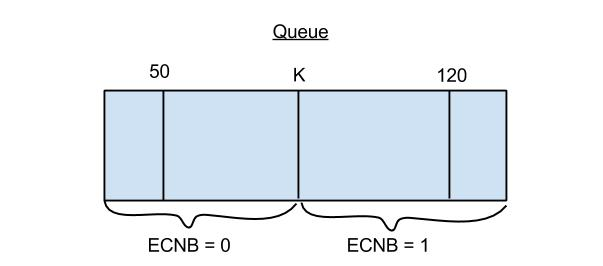
\includegraphics[width=3in, height=2.2in]{Queue4.jpg}
\caption{\textbf{The Queue for images}}
\end{figure}

\noindent When a node has a queue length greather than k, then it will advertise that it is congested by sending
a ECNB packet to all its neighbors. k is initialized for every node as 100. The way that k is changed depends 
on the number of neighbors around the current node and whether a packet was dropped or not. If a packet is
dropped, it must not be informing quickly enough to its surrounding nodes about this, therefore decrease to half 
between wherever k is and 50:

$$ k = max\{50, \frac{k + 50}{2} \}$$

\noindent Every two scans we will adjust the value k. The first link to the path were you are rounting packets
roughly determines the emptying rate. Therefore, depending on the percentage change of the value of this link, 
we will determine how much you change your queue.
\\

\noindent If the percentage change is positive then it means we expect to send less packets, so the rate of packets
leaving the queue is expected to decrease, so decrease the value of k:

$$ k = max\{50, k -  \frac{|\frac{1}{p_{new}} - \frac{1}{p_{old}}|}{\frac{1}{p_{old}}}|k - 50|   \}$$ 

\noindent If the percentage change is negative then we expect to see the rate of emptying the queue increase, therefore k is increased:

$$ k = min\{120, k +  \frac{|\frac{1}{p_{new}} - \frac{1}{p_{old}}|}{\frac{1}{p_{old}}}|k - 120|   \}$$ 

\subsection{Authentication}
When designing a communication system for first responders, its important that first responders are able to trust the messages they are receiving from fellow first responders. Therefore it is important to establish a mechanism by which first responders can authenticate “benign” messages (i.e. messages not sent by a malicious adversary). In the protocol presented in this paper, we use the RSA public-key cryptosystem to generate private and public-keys that will be used to authenticate messages. From here on, we use the term node and first responders interchangeably.

\subsubsection{Initialization}
During initialization, each node is assigned a public/private key pair by the base. Each node constructs a table with the following information for every node, and distributes it across all the nodes:

\begin{enumerate}
  \item The node's public-key. 
  \item The node's most recent message ID, initially 0.
\end{enumerate}

\subsubsection{Authentification Table}
Recall that everyone will have a table with an entry for each ally node. The table will contain two important numbers for each node: the node's public-key and the node's latest message ID number. The latest message ID number is a counter-like number inserted to every message a node sends such that each node can idenfity duplicate messages and be protected from malicious nodes trying to plot replay attacks. Consider Table 1 for a depiction of this table:

\begin{table}[ht]
\caption{Authentication Table} % title of Table
\centering % used for centering table
\begin{tabular}{c c c } % centered columns (4 columns)
\hline
\hline %inserts double horizontal lines
First Responder ID & Public-Key & Latest Message ID  \\[0.5ex] % inserts table
%heading
\hline % inserts single horizontal line
0 [base] & 69 & 669\\
1 & 50 & 837\\
% inserting body of the table
2 & 47 & 877 \\
3 & 45 & 300\\ [1ex]
% [1ex] adds vertical space
\hline
%inserts single line
\end{tabular}
\label{table:nonlin}
% is used to refer this table in the text
\end{table}

\subsubsection{Signatures}

Nodes should accept messages only from fellow first responders. 
To achieve this security, nodes sign their messages with their private-key. 
Consider the following function that signs messages:

$$\textsc{SIGN}(message, my\_private\_key, new\_message\_ID) = \sigma_{A}$$

\noindent The function returns a binary string $\sigma_{A}$, corresponding to the output of signing a message with the node's secret key. Since each private key assigned for each node is unique, each other node will need the corresponding public key to verify the signature. Since we also want to be protected from replay attacks, the message ID is incremented for each sent message.

\subsubsection{Authentication Mechanism}
Nodes can verify the validity of a message by using the following verification function:

$$\textsc{VERIFY}(signature, cooresponding\_public\_key) =  b $$

\noindent The output of $\textsc{VERIFY}$ will be a boolean, true, if the verification passes with that public-key or false if it fails. 
If the verification fails, then the message will be dropped and will not be forwarded.
\\
\noindent The receiving node uses the Authentication Table to decide which public key to use in order to authenticate a message.
When forwarding messages, nodes re-sign the contents of the message with their own private key.
\\

\noindent Once the authentication has passed, then the node will use the following function to get the message:

$$\textsc{GET\_MESSAGE}(message, corresponding\_public\_key) = m$$
\\

\noindent This function returns the corresponding message when applying the inverse of the sign function using the appropriate public-key.

\subsubsection{Dealing with replay attacks}

Another problem arises when a malicious node overhears a properly signed message and attempts to flood the network  with that message. This is a specific man-in-the-middle attack known as a replay attack. Our protocol prevents this by maintaining a counter, $message_ID$, at each node. This counter is increased before a message is sent. Therefore the format of a message looks like this:

$$message = (message\_information, \ message\_ID)$$

\noindent After \textsc{VERIFY} validates that the current message indeed was sent at one point by a trusted node, 
it will then check that the message ID number is not outdated. This is accomplished by the following procedure 
(given the node number and message ID):
\\

$def \ check\_ID\_number(node\_number, current\_message\_ID)$ \\
\hspace*{10 mm} $latest\_ID\_number\_from\_table = this.authentication\_table[node\_number].get\_Latest\_Message\_ID();$
\hspace*{10 mm} $if \ (current\_message.ID > latest\_ID\_number\_from\_table):$\\
\hspace*{20 mm} $this.authentication\_table[node\_number].update\_Latest\_Message\_ID(current\_message\_ID)$\\
\hspace*{20 mm} $return \ true$ \\
\hspace*{10 mm} $else:$\\ \ 
\hspace*{20 mm} $return \ false$\\


\subsubsection{Scalability and Updating the Authentication Table}

It is possible that a new node will be added to the network after the deployment. 
Therefore, it is important that other nodes are able to add new these new nodes to their Authentication Table.
\\

\noindent We address this by using the base as a trusted authority. The new node is required to report to the base
to obtain its own public and private key, as well as all of the public keys of the nodes already in the network.
\\

\noindent After this step, the base sends a special message (that it signs) and distributes the new public-key across the network. 
Then, the nodes forward the message, re-signing it each time, until every node has inserted the new public key of the new node into their table.

\section{Analysis}

\subsection{802.11}
The reason 802.11 is a good design decision is because it is a tested protocol that has evidence of being successful. Furthemore, it adds to the simplicity of the deisgn by re-using good protocols. It eliminates the hidden node problem because it always senses before sending. However, even though it is not optimal for the exposed node problem, we are designing under the design principle of optimizing for the most common case. Therefore this trade-off is not very significant because that case does not happen that often and the other benifits already mentioned.

\subsection{Routing protocol}

As mentioned previously, our link-state scheme has both advantages and disadvantages compared to alternative protocols
such as distance vector. Overall, the analysis will show why a link-state-based protocol is preferable. The initial
setup cost of our protocol is greater than that of a distance vector based one, both consuming more network bandwidth
and requiring more time to converge. However, at each update interval, link-state only requires that new changes
be broadcast across the network, whereas distance vector will flood the network, simultaneously calculating the 
best path and updating every node's routing information. Given the relatively low speed of first responders, we 
conclude that the average network topology change over an advertisement interval is small. Therefore, link-state is
preferable because the average amount of information link-state will broadcast at each update interval in a real world
scenario is less than that of distance vector.
\\

\noindent Our design is also robust against topology changes between update intervals. Our protocol is designed to react
to major changes in topology by sending LSAs as soon as a change is detected. Because each node has a complete view of 
the network topology, each node can locally recompute the best route to the base as soon as it hears a link or node has 
been lost, updated, or added. A distance-vector protocol would be unable to recompute new routes to the base station
between update intervals because any updates to routing information need to be initiated from the base node.
\\

\noindent Finally, every link-state advertisement is broadcast to every node in the network. Resultantly, the base
will hear every link-state advertisement originating from a connected node. Our design takes advantage of this fact by
bundling GPS information on each node into its link-state advertisement. This optimization, available only to link-state
based protocols, simplifies our cost metric and fulfills a system requirement. 

\subsection{Authentication}
Under the assumption that the base and legitimate nodes are all trusted, the authentication system presented is extremely secure. This is because during the initialization phase, everyone obtained a secure key from the trusted authority (the base). Therefore, if no new first responders join the network, every node in the network so far will be able to verify and sign every message that it receives or sends. \\

\noindent However, we can not ignore the potential scalability problem of this initial design. Therefore, our design also accounts for adding new nodes to the network. As explained above, these new nodes undergo a similar procedure for obtaining keys from the trusted base. The rest of the nodes will not accept messages from this node until the base distributes the new node's public key. The old nodes will trust this new key, as the message containing it was signed by a trusted key.
\\

\noindent Since the private keys are generated with RSA, the probability that a malicious node guesses a key and is able to find a colliding signature is negligible (given the intractability of factoring large numbers). The keys used for RSA are usually of length 2048 bits, so the probability that a key generated by a malicious node a collides with an already generated private key is $2^{-2048}$. This case is extremely unlikely, but in a huge network where this could be a problem, the number of bits used for key generation could be increased.\\

\noindent The authentication mechanism presented is also secure against replay attacks. Since the message ID is included in the message signature, it is not enough for a malicious node to simply guess an incremented message ID, as it would have to resign the message accounting for the new key. This is unfeasable, given that the malicious node can not guess the nodes' private keys.

\subsubsection{Throughput for sending images}

The idea for the throughput algorithm is very simple, as long as you can push more packets through your best route, keep doing that (to achieve highest throughput). However, when congestion becomes a problem, inform you neighbors, and then your neighbors will mark packets that should be re-routed. When node get re-routing packets, they will again run Dijkstra, but instead not consider any paths that the algorithm considers congested. Another quintessential point to note about the algorithm is that it does not re-route packets to nodes were there would be interference. The reason for this is that, nodes that are close to each other interfere with each other if they send packets at the same time. Therefore, if one wants to achieve good throughput and real parallelism when sending packets, its better to consider re-routing paths such that the amount of intereference with congested sections of the network are minimized. Therefore, this algorithm attempts to maximize actual realizable throughput by re-routing to paths with high throughput ,low congestion and low interference.


\subsection{Use cases}

\subsubsection{Use more resources than necessary}

There are two scenarios in which the system uses more resources than necessary. First, a packet may follow an optimal path
to the base for a number of hops, only to find that a link on its path has died. The node will broadcast an advertisement
and the packet will then be rerouted after it has already followed a path for a number of hops, which uses more additional
resources. Secondly, after a link fails to send a packet a number of consecutive times, the sending node will call
\textsc{scan}. However, it is possible the probability of the link has not changed and the sending node was unsuccessful.
The \textsc{scan} in this scenario uses more resources than necessary to deliver a packet.

\subsubsection{Failure to inform the base within 5 minutes}

AdHocPro may fail to inform the base of a node $n$'s location within 5 minutes only if all nodes which have received an
advertisement from $n$ become disconnected from the network before the advertisement reaches the base. The broadcast
nature of LSAs makes failure to inform the base of every connected node's location highly unlikely.

\subsubsection{Malicious node preventing a message}

A malicious node may always prevent a message from reaching the base by jamming the network with messages. Doing so prevents
other nodes from sending their messages due to 802.11 MAC.

\subsubsection{Behavior under different loads}

\subsubsection{Light traffic}

The current algorithm choses alternative routes when congestion is high. Therefore, under the assumption that all wirless links interfere and only one link can send at a time and that queues are low (or mostly emmoty), the actual throughput is inversely proportional to the suggested metric:

$$  Total \ Expected \ Transmition \ Cost = \sum_{i=0}^{k}\frac{1}{p_{i}}$$

Therefore, the current algorithm will choose the maximum throughput under this case. One can think that the assumption that all link interfere are a bit strong, but considering that the uppder bound on radius of transmission is as high as a 20 metere building or 50 meteres in the longest case, this assumption actually not very unrealistic. However, because we are using 802.11, interference will not be a problem and if two link want to send at the same time and are separeted enough, this will still be possible.

\subsubsection{Medium traffic}

The case for medium traffic is similar to light traffic. Since the threshold is initiated at a relitavely large value, 100 packets, then it will take a while until a path gets congested and get rerouted to potentially suboptimal paths. Furthermore, the threshold is changing approximately proportionally to the changes in emptying rate, therefore, if the emptying rate changes drastically, the threshold value should change to reflect that.

\subsubsection{Heavy traffic}

Under heavy traffic conditions the behaviour of the algorithm is more complicated. However, what it will try to do is re-route packets through paths that have the next highest expected throughput. If congestion is high, then it will start distributing the loads to other nodes, which is good. Furthermore, it will try to distribute it to nodes that are not in interfering paths with currently congested nodes. This is important because there is no point in distributing the load, if only one link at a time can be used and the alternative path has lower throughput. The reason for this is that there will be no real parallelism. This is positive but comes at a cost. It will have to re-compute new paths for re-routing without the current congested nodes. This will cost the node $O(E + VlogV)$ computation time. However, it could potentially get parallelism in routing to the base and higher throughput. If throughput is extremely high and there are not ways to re-route successfully, then this algorithm will just decrease the contention window, which is the best it can do with the current state of the network.

\subsubsection{Replay attacks}

Our system is robust against replay attacks, as described in the ``Authentication" section. Using the Authentication Table, 
nodes can quickly determine that a message is a replay of a previously heard message using the message IDs. However, 
a replay attack will still use network bandwidth and cause more losses of legitimate packets, which is something we cannot prevent.

\subsubsection{Hop bypassing}

If a node $k$ overhears a message that is intended for node $j$, it will drop the message, even if $k$ is closer to the base than $j$.
Even though ignoring the message header in this case would increase throughput, in general, ignoring \textsc{send} headers will quickly cause
the protocol to break down. The routing system works on the assumption that the route calculated for a packet is the route the packet
actually takes. Without this representation invariant, a node might incorrectly think a route no longer exists, and LSAs may be sent 
mistakenly, all of which decreases throughput in the long run. Thus, we sacrifice a small increase in throughput for an edge case in
favor of simplicity of the protocol and long-term consistency of the \textsc{update} and \textsc{send} procedures. We also note that 
this would never occur for location information, as GPS coordinates are transmitted through an LSA broadcast instead of \textsc{send}. 

\section{Conclusion}

AdHocPro is a stable and complete solution for ad-hoc networks when it is bundled with 802.11. Our systems allows first responders to
focus on their mission without worrying about their ability to communicate with their base camp. By thwarting potentially malicious
users and effectively delivering location and images across the network, AdHocPro uses novel methods to provide a seamless user experience.

\section{References}

\end{document}
